% Chapter Template

\chapter{Inference using HUSJR data} % Main chapter title

\label{Chapter:Inference} % Change X to a consecutive number; for referencing this chapter elsewhere, use \ref{ChapterX}

In this chapter is presented a study done with the collaboration of a team of ophthalmologists of Tarragona province with images collected during 8 years at \emph{Hospital Universitari Sant Joan de Reus (HUSJR)} in the framework of the Spanish project PI15/01150. The results show that the original model trained with EyePACS, after being fine-tuned for the prediction of classes, following the Messidor-2 standard, is able to predict with a high confidence the ophthalmologists' classifications.

%----------------------------------------------------------------------------------------
%	SECTION 1
%----------------------------------------------------------------------------------------

\section{Introduction}

Machine Learning paradigm allow computer systems the ability to learn from data. These algorithms permit the identification of the most relevant features and the way of combining them to maximize the performance in a particular classification or regression problem. Identifying such a set of important features enables the generalization of prediction capabilities of the designed models. %Feature vectors are also known as co-variates in statistical jargon. That’s why co-variate shift could be expressed as feature vector shift in machine learning jargon.

%Model design in Machine Learning is done using a data set that is split in two main parts: a train set and a test set. Due to the way of choosing both sets, ie. random selection, we assure that they come from the same population and share the same probability distribution.

After the training process we usually want to use the model for inference over different data. New data can share a priori most of the properties of data used in training, but also it may have distinctive properties not present in the original data that could influence on the classification, ie. the probability distributions of both populations can be similar but also have some differences. Therefore, before applying inference over this new data, it is important to check for the existence of distinctive elements affecting the classification/regression performance. If this happens, we say that there is a dataset shift between both populations producing a co-variate shift in the model derived features used for prediction by the model \citep{sugiyama2017dataset}. Detecting or discarding such a co-variate shift is critical when using models from prediction in similar but different populations.

Exploratory Analysis using Graphical Methods are a very good way of detecting the class separation quality. Feature-space domains are frequently highly correlated spaces that can be compressed into lower dimensional space representations. The shape of the internal representation of the data manifold determines the effectiveness of the dimensionality reduction method. In cases where the manifold holds a linear representation, methods like Principal Components Analysis (PCA) \citep{pearson1901principal}, Multidimensional Scaling (MDS) \citep{kruskal1964multidimensional} or Independent Components Analysis (ICA) \citep{hyvarinen1999fast} can be very effective. In cases where the manifold is non-linear or the points are to close to each other, non-linear techniques like Isometric Mapping (ISOMAP) \citep{tenenbaum2000global} or t-distributed Stochastic Neighboring Embedding (t-SNE) \citep{maaten2008visualizing} are more effective. %or Uniform Manifold Approximation (UMAP) can be more effective. \cite{van2009dimensionality}. 

For visualization purposes the objective is to find a method that is able to separate diverging points and to cluster those with similar properties in a two-dimensional or three dimensional space. Even in cases where the manifold can be linearly compressed into a smaller representation, if the dimensions are more than three, it does not allow visualization, requiring the usage of non-linear methods to reduce even more the dimensionality to two or three dimensions. 

t-SNE is a very effective visualization method that, with the proper selection of parameters, is able to separate effectively the different classes present in the manifold. t-SNE uses an optimization algorithm to minimize the Kullback-Leibler divergence \citep{kullback1951information} between two probability distributions, one in the original multidimensional space and another one in the visualization space. Variables to optimize are the distance between points in the visualization space. 

Therefore, we will use t-SNE for the analysis of the dataset provided by HUSJR. We also have, in this case, the assistance of the ophtalmology team of this hospital. So, we defined a four-step methodology for the testing of the classification model using their dataset. The description of this dataset can be found in chapter \ref{Chapter:Background}.


\iffalse % begin of commented part

\subsection{Probability distribution distance testing}

One quantitative way of testing for the absence of co-variate shift is considering different the probability distributions of training and inference populations and calculating the distance between them. Kullback-Leibler divergence or its generalization in the form of f-divergences \citep{ali1966general} are a way for computing the distance between two distributions. A threshold is defined and the distance is computed using a sample based approximation. In case of being the distance greater than the threshold, co-variate shift is present. In case of being the distance lower than the threshold co-variate shift can be discarded. Table \ref{tab:f_divergences} show a list of some of the divergences that can be used for calculating the distance between distributions.

\begin{table}[h!]
	\centering
	\resizebox{\columnwidth}{!}{ 
		\begin{tabular}{l|c}
			Name             & $ D_f(P \mid \mid Q) $ \\
			\hline		
			Total variation  & $\frac{1}{2}\int \mid p(x)-q(x)\mid dx$ \\
			Kullback-Leibler & $\int p(x) \log \frac{p(x)}{q(x)}dx $  \\
			Reverse Kulback-Leibler  & $\int q(x) \log \frac{q(x)}{p(x)}dx $ \\
			Pearson $\chi^2$       & $\int \frac{(q(x)-p(x))^2}{p(x)}dx$ \\
			Neyman $\chi^2$        & $\int \frac{(p(x)-q(x))^2}{q(x)}dx$  \\
			Squared Hellinger        & $\int (\sqrt{p(x)}-\sqrt{q(x)})^2 dx$ \\
			Jeffrey                  & $\int (p(x) - q(x))\log \left(\frac{p(x)}{q(x)}\right)dx)$ \\
 			Jensen-Shannon           & $\frac{1}{2}\int p(x) \log \frac{2p(x)}{p(x)+q(x)} + q(x) \log \frac{2q(x)}{p(x)+q(x)} dx$ \\
			Jensen-Shannon weighted  & $\int p(x) \pi \log \frac{p(x)}{\pi p(x)+(1-\pi)q(x)} + (1-\pi)q(x) \log \frac{q(x)}{\pi p(x)+ (1-\pi) q(x)} dx$ \\
			GAN                      & $\int p(x) \log \frac{2p(x)}{p(x)+q(x)} + q(x) \log \frac{2q(x)}{p(x)+q(x)} dx - \log 4 $ \\
			$\alpha$-divergence    & $ \frac{1}{\alpha (\alpha - 1)} \int \left(p(x) \left[\left(\frac{q(x)}{p(x)}\right)^{\alpha} - 1\right] - \alpha (q(x) - p(x))\right)dx $ \\ 			
			\hline
		\end{tabular}
	}
	\caption[Summary of f-divergences]{Summary of f-divergences available for measuring the distance between two probability distributions $P$ and $Q$ }
	\label{tab:f_divergences}
\end{table}

\subsection{Non-randomness testing}

Another quantitative way of detecting co-variate shift is testing for the presence of non-randomness on the data. In case that both samples belong to the same distribution, no presence of differences in the data belonging to the same classes should be detected. In case both samples belong to different populations some kind of differential structure in the data can be detected. One test used extensively for this purpose is the Wald-Wolfowitz test.

\fi % end of commented part

\section{Methods}

In this section we present the method that is used for adapting the model trained with the EyePACS model to the HUSJR population. 

The steps required for model adaptation can be summarized in: model evaluation, standardization of categories, model and dataset adaptations and final evaluation.

\subsection{Original model evaluation}

In this phase disease experts check the model predictions over the test set of the original model. The first thing that has to be checked is the compatibility between class output definition in the original model with the classes defined in the objective data set. If differences in class definition are identified, they must be taken into account because it would require a retraining of the model. This first step allows also the evaluation of the predictions quality and to have a qualitative evaluation on original model test images.

\subsection{Category standardization}

The objective of this part is comparing if the categorization used in original model is the same that is required in the target population. Sometimes, categories can be interpreted in slightly different ways if the definition is more precisely established. This happens in medicine where subjectivity appears. If differences are detected, they require some adaptation either in the target class or in the model class definitions.

\subsection{Model and dataset adaptations}

If evident discrepancies are detected, class re-definitions in original model and target population should be applied, requiring either retraining in model or relabeling in target population. If model classes are redefined, the model must be retrained. If changes are mild, probably a last layer classification retraining will suffice. If evaluation function results are not optimal, deep changes are required, ie. a full network retraining.

\subsection{Final evaluation}

Finally, the modified dataset is tested with the classification model in order to validate it. Having possible qualitative and quantitative results, the final model can be used for inference in the new objective population.

\section{Results}

%\subsection{Data}

%The data used is described in section \ref{dataset:reus}. 

In this section we present the results of the four steps proposed for analyzing the HUSJR dataset.

\subsection{Original model evaluation}

The first important difference between model and the new population is the categorization employed. Original model is designed for differentiation of 5 classes. HUSJR population distinguishes between only 4 classes. Expert analysis over images of the original data set indicate that, HUSJR classification groups together class 3 and 4 of the original model. 

Two tests are done in order to have a initial evaluation of the performance of the model: 

Firstly, an evaluation of all images is done using the original DCNN model. Table \ref{inf:fig:confusion_original} shows the results obtained of the classification. Calculated QWK index is 0.791 for 4 classes (grouping class 3 and 4). This value is about 1,6\% lower than the achieved for the EyePACS test set, ie. $QWK = 0.804$ and a 5\% lower than the achieved for Messidor-2 Dataset of the original model ($QWK=0.831$).


\begin{table}[ht]
	\centering
	\scalebox{0.85}{
		\begin{tabular}{c|ccccc}
			\hline
			        & Pred 0 & Pred 1 & Pred 2 & Pred 3 & Pred 4\\ \hline
			True 0 &  15,112 &   2,024 &     159 &      6  &      12\\ 
			True 1 &      11 &     547 &     326 &     14  &       3\\ 
			True 2 &       0 &       4 &     439 &    133  &       7\\ 
			True 3 &       0 &       1 &      20 &    358  &      54\\ 
			\hline	
		\end{tabular}
	}
	\caption[CM of HUSJR data using EyePACS trained model]{Confusion matrix of predicted classes vs classes given by HUSJR with EyePACS trained original model. $QWK = 0.791$ (Grouping together class 3 and 4)}
	\label{inf:fig:confusion_original} 
\end{table}

Secondly, t-SNE is used for visualizing the feature-space vector representation of each image. Figure \ref{inf:fig:featspace} shows a two-dimensional t-SNE visualization of the feature space. Each point representing an image and point color representing the tagged class. We can see a gradation separation between classes very similar to the observed in original and in Messidor datasets. 

\begin{figure}[!htb]
	\centering
	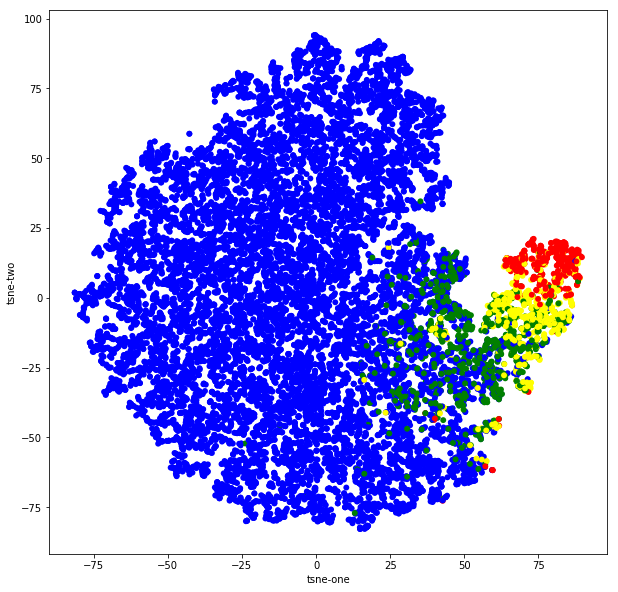
\includegraphics[width=0.8\textwidth]{Figures/chapter_reus/feature_space_reus.png}
	\caption[Feature space visualization of HUSJR dataset]{t-SNE visualization of the feature space representation of samples of HUSJR dataset. Blue points represent class 0 images, green points class 1, yellow points class 2 and red points class 3}
	\label{inf:fig:featspace}
\end{figure}


\subsection{Category standardization}

Due to the differences observed between the original classification and the new one, HUSJR experts decide to use as a standard classification the defined one in Messidor-2 database \citep{decenciere_feedback_2014}. In this categorization, only four classes are defined. HUSJR sample is reviewed to adapt the original classification to the new defined standard. 

\subsection{Model adaptation}

Original model is designed as a combination of a fully convolutional neural network that acts as a feature extractor. Features are linearly combined for classification. Messidor-2 last layer feature vectors are calculated. A new linear classifier is trained using these features for the prediction of new standardized classes. The combination of original feature extractor with the new last linear layer is used as a new prediction model for calculation of the new predicted classes of the HUSJR sample.

\subsection{Results re-evaluation}

The new confusion matrix obtained for HUSJR is presented in table \ref{inf:fig:confusion_new}.

\begin{table}[ht]
	\centering
	\scalebox{1.0}{
		\begin{tabular}{c|ccccc}
			\hline
			& Pred 0 & Pred 1 & Pred 2 & Pred 3\\ \hline
			True 0 &  15,277 &   1,944 &      83 &      9 \\ 
			True 1 &       5 &     595 &     284 &     17 \\ 
			True 2 &       0 &       2 &     456 &    125 \\ 
			True 3 &       0 &       1 &       6 &    426 \\ 
			\hline	
		\end{tabular}
	}
	\caption[CM of HUSJR data using EyePACS trained model finetuned with Messidor]{Confusion matrix of predicted classes vs original classes (HUSJR Dataset) with EyePACS trained original model plus a linear classifier retrained using Messidor Dataset. $QWK = 0.823$}
	\label{inf:fig:confusion_new} 
\end{table}

QWK inter-rater agreement evaluation index obtained ($QWK=0.823$) is similar to the reached between ophthalmologist experts in disease detection. 

The indexes obtained for classification of the most severe cases of the disease (considering positive class = 2,3 and negative class = 0,1) are:

\begin{itemize}
	\item Sensitivity = 0.997
	\item Specificity = 0.978
	\item Positive predictive value (PPV) = 0.720
	\item Negative predictive value (NPV) = 0.9998
	\item False negative rate (FNR) = 0.003
	\item False positive rate (FPR) = 0.022
	\item False discovery rate (FDR) = 0.280
	\item False omission rate (FOR) = 0.0001
	\item Accuracy (ACC) = 0.979
	\item $F_1$ Score = 0.836
	\item Matthews correlation coefficient (MCC) = 0.838
	\item Bookmaker Informedness (BM) = 0.975
	\item Markedness (MK) = 0.720
\end{itemize}

$Sensitivity$ obtained is greater than $0.99$ and $Specificity$ near $0.98$ for the detection of the most severe cases of the disease. These and all the other indexes prove experimentally that the model is able to predict with high confidence the correct values of the disease for the new population of study.

\section{Conclusions}

In this chapter, it is studied the applicability of our best model for the prediction of diabetic retinopathy, trained using the EyePACS dataset, for the prediction of diabetic retinopathy in HUSJR. A feature space visualization has been done in order to check its capacity for separating between classes. After checking that the separation was done properly, a first evaluation of the model predictability was done, obtaining good results, but with small loss in performance. This loss was probably produced to the slight differences in class definitions. After its standardization, the linear classifier of the model was retrained using Messidor-2 Dataset, using as a feature extractor the original model. Performance of the new model was tested again, reaching values of inter-rater agreement similar to the obtained by expert ophthalmologists. Classification indexes for the detection of the most severe cases of the disease are also presented, showing excellent performance also over the new population. Modified model is ready to be used for inference over the new population. Medical team is extremely satisfied with the results. Dr. Pere Romero, head of Ophthalmology Unit at HUSJR confirms that the quality of the classification is good enough to be used in a near future.
